\section{Introduction}
In this chapter we will discuss on social and ethical impact, result, performance and accuracy of this system. We took many test case result and we will discuss on it.

\section{Dataset Description}
We tried to find the evaluation of our developed system. We tested for thirty times and we monitored the delay of every modules and features with stopwatch. We did black box testing. We recorded this delay in second format in excel sheet. Table \ref{delay_table} represents the delay value recorded in excel sheet. In this table in the first column "Key matched and gate opened time" is the time to submit pin code and opening gate after matching pin. In the second column "Car parking time" is the time to park the car at slot after matching pin and opening gate. In the third column "Park data update time" is the time to update parked state at server. In the fourth column "Alarm triggering time at Android" is the time to ring alarm at android phone after placing car from parked state. In the fifth column "Alarm triggering time at Device" is the time to ring alarm at system after placing car from parked state. In the sixth column "Sms sending time" is the time to coming message using GSM module at mobile phone after placing car from parked state. In th seventh column "Unpark and gate open time" is the time to open gate after requesting for unpark from android application. In the Eighth column "Unpark data update time" is the time to update state at server after unparking car. In the ninth column "Total time" is the time of every cycle. In the tenth column "Used Slot" indicates that in which test case which parking slot is used. 

% Please add the following required packages to your document preamble:
% \usepackage{graphicx}
\begin{table}[H]
\centering
\caption{Delay of Modules From Thirty Test Case}
\label{tab:my-table}
\resizebox{\textwidth}{!}{%
\begin{tabular}{|c|c|c|c|c|c|c|c|c|c|c|}
\hline
\textbf{\begin{tabular}[c]{@{}c@{}}Test\\ case\\ No.\end{tabular}} & \textbf{\begin{tabular}[c]{@{}c@{}}Key \\ matched \\ and   \\ gate \\ opened \\ time\end{tabular}} & \textbf{\begin{tabular}[c]{@{}c@{}}Car \\ parking \\ time\end{tabular}} & \textbf{\begin{tabular}[c]{@{}c@{}}Park  \\ data \\ update \\ time\end{tabular}} & \textbf{\begin{tabular}[c]{@{}c@{}}Alarm \\ triggering \\ time \\ at\\ Android\end{tabular}} & \textbf{\begin{tabular}[c]{@{}c@{}}Alarm \\ triggering \\ time \\ at \\ device\end{tabular}} & \textbf{\begin{tabular}[c]{@{}c@{}}Sms \\ sending \\ time\end{tabular}} & \textbf{\begin{tabular}[c]{@{}c@{}}Unpark \\ and \\ gate \\ open \\ time\end{tabular}} & \textbf{\begin{tabular}[c]{@{}c@{}}Unparking \\ data \\ update \\ time\end{tabular}} & \textbf{\begin{tabular}[c]{@{}c@{}}Total \\ time\end{tabular}} & \textbf{\begin{tabular}[c]{@{}c@{}}Used \\ Slot\end{tabular}} \\ \hline
1 & 2 & 19 & 62 & 3 & 6 & 11 & 5 & 16 & 124 & 4 \\ \hline
2 & 2 & 20 & 65 & 3 & 7 & 10 & 5 & 18 & 130 & 3 \\ \hline
3 & 1 & 18 & 57 & 2 & 5 & 0 & 4 & 15 & 102 & 1 \\ \hline
4 & 2 & 17 & 59 & 3 & 6 & 9 & 5 & 17 & 118 & 2 \\ \hline
5 & 2 & 20 & 64 & 4 & 5 & 11 & 4 & 16 & 126 & 2 \\ \hline
6 & 2 & 16 & 59 & 2 & 5 & 10 & 6 & 15 & 115 & 4 \\ \hline
7 & 1 & 18 & 58 & 3 & 5 & 10 & 4 & 15 & 114 & 3 \\ \hline
8 & 2 & 17 & 62 & 3 & 6 & 10 & 5 & 15 & 120 & 3 \\ \hline
..... & .................... & .................... & .................... & .................... & .................... & .................... & .................... & .................... & .................... & .................... \\ \hline
30 & 1 & 16 & 61 & 3 & 6 & 8 & 4 & 18 & 117 & 4 \\ \hline
\end{tabular}%
}
\label{delay_table}
\end{table}




\section{Impact Analysis}
Our developed smart car parking system can have some impact such as social, environmental and ethical impact. In this section we are discussing most probable impact of this system. Some social and environmental impacts given below:

\subsection{Social and Environmental Impact}
\begin{itemize}
    \item This system needs continuous electricity supply. Thus is consumes electricity
    \item This device consumes internet data
    \item If any sensor damaged this system will behave wrongly
    \item If servo motor damaged user will get in stack
    \item If breaks the firewall and access to database, it will be terrifying
    \item This system makes human lazy
    \item This system will decrease the use of cash 
\end{itemize}

\subsection{Ethical Impact}
Every technology has the power to do task smartly, firstly and accurately. It depends on human who is the user of the technology. If user use it for welfare it will be blessing but if use it for destructive it will be harmful. As usual this system can have some ethical impacts. Some impacts are given below:
\begin{itemize}
    \item This smart car parking system can make care taker jobless.
    \item People will get dependent on automated system
    \item This smart system will dominate non smart parking system.
\end{itemize}

\section{Evaluation of Framework}

\subsection{Visualization of Delay Data}
We plotted those recorded value of thirty test cases in excel sheet. In figure \ref{chart_} we see that among 30 test cases for only two times we got nothing. Those two times it made lower spike. We splat a full cycle into eight modules. We measured each modules working time with stopwatch and we plotted into excel.

\begin{figure}[H]
\centering
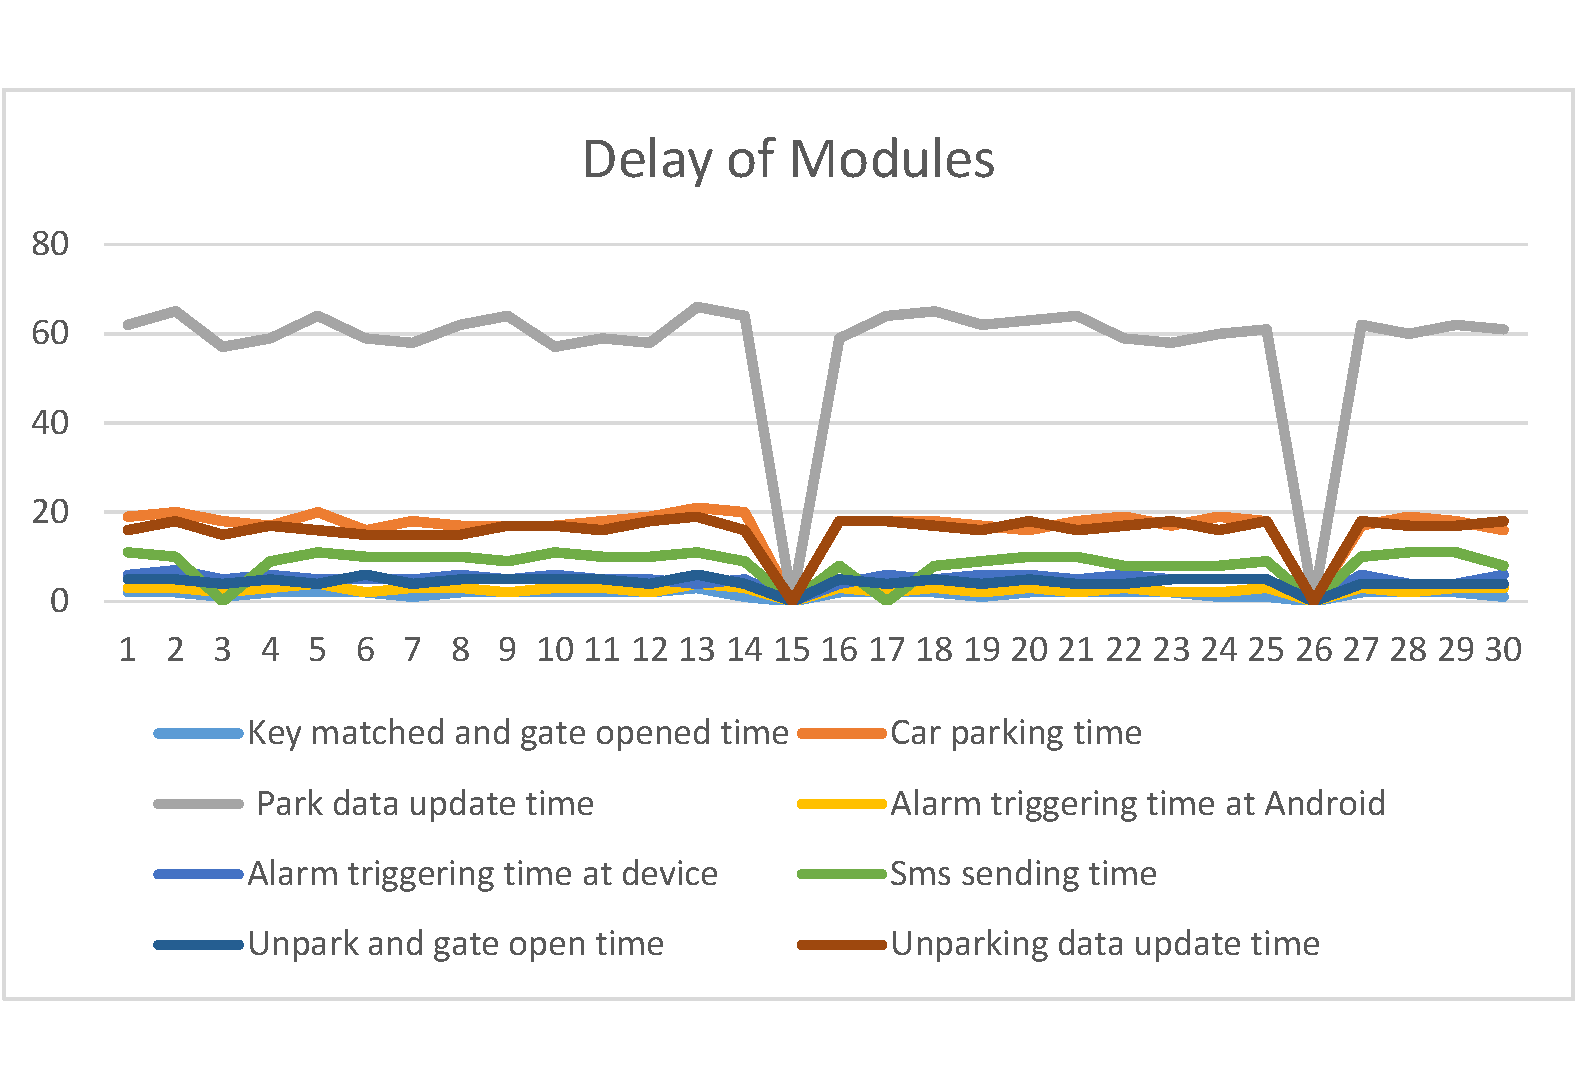
\includegraphics[width=0.9\textwidth]{figures/chart.pdf}
\caption{Plotting of working time of modules}
\label{chart_}
\end{figure}

\subsection{Emergency vs Non-Emergency Working Cycle Time}
We tried to calculate the working cycle period of parking at emergency and non emergency slot system. We found the working time of modules those are given below:

% Please add the following required packages to your document preamble:
% \usepackage{graphicx}
\begin{table}[H]
\centering
\caption{Emergency vs Non-Emergency slot Working Cycle}
\label{tab:my-table}
\resizebox{\textwidth}{!}{%
\begin{tabular}{|l|c|c|c|c|c|c|c|c|c|}
\hline
\textbf{\begin{tabular}[c]{@{}l@{}}Test\\ Case\\ No.\end{tabular}} & \textbf{\begin{tabular}[c]{@{}c@{}}Key\\  matched\\  and  \\  gate \\ opened\\  time\end{tabular}} & \textbf{\begin{tabular}[c]{@{}c@{}}Car \\ parking \\ time\end{tabular}} & \textbf{\begin{tabular}[c]{@{}c@{}}Park  \\ data \\ update \\ time\end{tabular}} & \textbf{\begin{tabular}[c]{@{}c@{}}Alarm \\ triggering \\ time \\ at \\ Android\end{tabular}} & \textbf{\begin{tabular}[c]{@{}c@{}}Alarm \\ triggering \\ time \\ at \\ device\end{tabular}} & \textbf{\begin{tabular}[c]{@{}c@{}}Sms \\ sending \\ time\end{tabular}} & \textbf{\begin{tabular}[c]{@{}c@{}}Unpark \\ and \\ gate \\ open \\ time\end{tabular}} & \textbf{\begin{tabular}[c]{@{}c@{}}Unparking \\ data \\ update \\ time\end{tabular}} & \textbf{\begin{tabular}[c]{@{}c@{}}Total \\ time\end{tabular}} \\ \hline
\textbf{Emergency} & 4 & 10 & 1 & 3 & 6 & 11 & 4 & 6 & 25 \\ \hline
\textbf{Non Emergency} & 2 & 20 & 65 & 3 & 7 & 10 & 5 & 18 & 110 \\ \hline
\end{tabular}%
}
\label{emer_vs_non}
\end{table}
From table \ref{emer_vs_non} we can see that the cycle period of parking at emergency slot is 25 second and non emergency slot is 110 second. 

\subsection{Slot Used Ratio}
From chart \ref{slot_used} we can see the used slot ratio of thirty test cases. Emergency slot or slot 1 is used for 2 times, slot 3 is used for 10 times and slot 4 is used for 7 times. From pricing distribution we can see that the fare of Emergency slot is 40 taka per hour, slot 2 is 30 taka per hour, slot 3 is 25 taka per hour and rest of the other slot is 20 taka per hour. 
\begin{figure}[H]
\centering
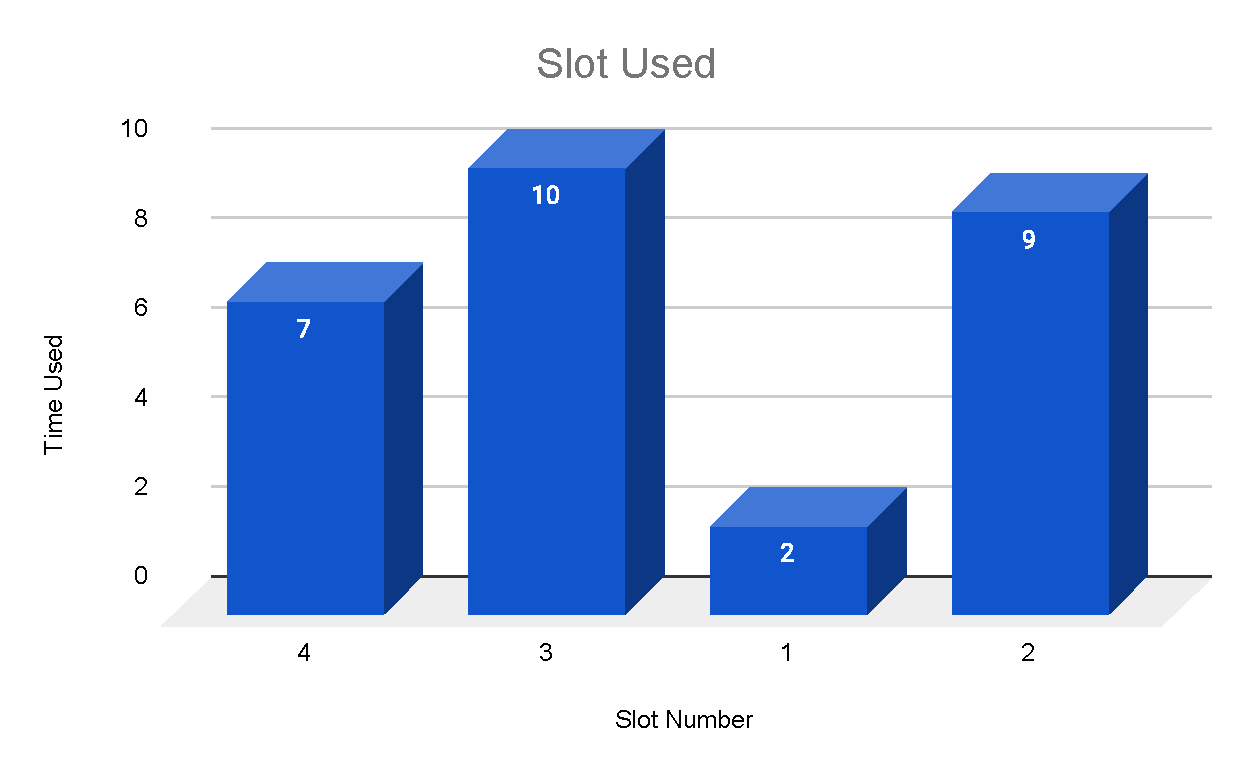
\includegraphics[width=0.9\textwidth]{figures/slot_used.pdf}
\caption{Slot Used Ratio}
\label{slot_used}
\end{figure}


\section{Evaluation of Performance}


\subsection{Accuracy Calculation}
We tested the total procedure for thirty times and we checked that every module and hardware components are working or not. We found result which is given below.
\begin{table}[H]
\centering
\caption{Accuracy of This System}
\begin{tabular}{|l|l|l|l|l|l|l|l|}
\hline
\textbf{Serial} & \textbf{Sensor}                                                & \textbf{LED}                                                   & \textbf{Keyboard}                                             & \textbf{Display}                                               & \textbf{Alarm}                                                & \textbf{SMS}                                                  & \textbf{Payment}                                              \\ \hline
1               & Y                                                              & Y                                                              & Y                                                             & Y                                                              & Y                                                             & N                                                             & Y                                                             \\ \hline
2               & Y                                                              & Y                                                              & Y                                                             & Y                                                              & Y                                                             & Y                                                             & Y                                                             \\ \hline
3               & Y                                                              & Y                                                              & Y                                                             & Y                                                              & Y                                                             & Y                                                             & Y                                                             \\ \hline
4               & Y                                                              & Y                                                              & Y                                                             & Y                                                              & Y                                                             & Y                                                             & Y                                                             \\ \hline
5               & Y                                                              & Y                                                              & Y                                                             & Y                                                              & Y                                                             & Y                                                             & Y                                                             \\ \hline
6               & Y                                                              & Y                                                              & Y                                                             & Y                                                              & Y                                                             & Y                                                             & Y                                                             \\ \hline
7               & Y                                                              & Y                                                              & Y                                                             & Y                                                              & Y                                                             & Y                                                             & Y                                                             \\ \hline
8               & Y                                                              & Y                                                              & Y                                                             & Y                                                              & Y                                                             & Y                                                             & Y                                                             \\ \hline
9               & Y                                                              & Y                                                              & Y                                                             & Y                                                              & Y                                                             & Y                                                             & Y                                                             \\ \hline
10              & Y                                                              & Y                                                              & Y                                                             & Y                                                              & Y                                                             & Y                                                             & Y                                                             \\ \hline
11              & Y                                                              & Y                                                              & Y                                                             & Y                                                              & Y                                                             & Y                                                             & Y                                                             \\ \hline
12              & Y                                                              & Y                                                              & Y                                                             & Y                                                              & Y                                                             & Y                                                             & Y                                                             \\ \hline
13              & Y                                                              & Y                                                              & Y                                                             & Y                                                              & Y                                                             & Y                                                             & Y                                                             \\ \hline
14              & Y                                                              & Y                                                              & Y                                                             & Y                                                              & Y                                                             & Y                                                             & Y                                                             \\ \hline
15              & Y                                                              & Y                                                              & N                                                             & Y                                                              & N                                                             & N                                                             & N                                                             \\ \hline
16              & Y                                                              & Y                                                              & Y                                                             & Y                                                              & Y                                                             & Y                                                             & Y                                                             \\ \hline
17              & Y                                                              & Y                                                              & Y                                                             & Y                                                              & Y                                                             & N                                                             & Y                                                             \\ \hline
18              & Y                                                              & Y                                                              & Y                                                             & Y                                                              & Y                                                             & Y                                                             & Y                                                             \\ \hline
19              & Y                                                              & Y                                                              & Y                                                             & Y                                                              & Y                                                             & Y                                                             & Y                                                             \\ \hline
20              & Y                                                              & Y                                                              & Y                                                             & Y                                                              & Y                                                             & Y                                                             & Y                                                             \\ \hline
21              & Y                                                              & Y                                                              & Y                                                             & Y                                                              & Y                                                             & Y                                                             & Y                                                             \\ \hline
22              & Y                                                              & Y                                                              & Y                                                             & Y                                                              & Y                                                             & Y                                                             & Y                                                             \\ \hline
23              & Y                                                              & Y                                                              & Y                                                             & Y                                                              & Y                                                             & Y                                                             & Y                                                             \\ \hline
24              & Y                                                              & Y                                                              & Y                                                             & Y                                                              & Y                                                             & Y                                                             & Y                                                             \\ \hline
25              & Y                                                              & Y                                                              & Y                                                             & Y                                                              & Y                                                             & Y                                                             & Y                                                             \\ \hline
26              & Y                                                              & Y                                                              & N                                                             & Y                                                              & N                                                             & N                                                             & N                                                             \\ \hline
27              & Y                                                              & Y                                                              & Y                                                             & Y                                                              & Y                                                             & Y                                                             & Y                                                             \\ \hline
28              & Y                                                              & Y                                                              & Y                                                             & Y                                                              & Y                                                             & Y                                                             & Y                                                             \\ \hline
29              & Y                                                              & Y                                                              & Y                                                             & Y                                                              & Y                                                             & Y                                                             & Y                                                             \\ \hline
30              & Y                                                              & Y                                                              & Y                                                             & Y                                                              & Y                                                             & Y                                                             & Y                                                             \\ \hline
Result          & \begin{tabular}[c]{@{}l@{}}(30-0)/30\\ *100=100\%\end{tabular} & \begin{tabular}[c]{@{}l@{}}(30-0)/30\\ *100=100\%\end{tabular} & \begin{tabular}[c]{@{}l@{}}(30-2)/30\\ *100=93\%\end{tabular} & \begin{tabular}[c]{@{}l@{}}(30-0)/30\\ *100=100\%\end{tabular} & \begin{tabular}[c]{@{}l@{}}(30-2)/30\\ *100=93\%\end{tabular} & \begin{tabular}[c]{@{}l@{}}(30-4)/30\\ *100=86\%\end{tabular} & \begin{tabular}[c]{@{}l@{}}(30-2)/30\\ *100=93\%\end{tabular} \\ \hline
\end{tabular}
\label{accuracy_table}
\end{table}
Table \ref{accuracy_table} represents the result and accuracy of our system. We found the accuracy of our system is 93\%.

\subsection{Result Analysis}
From table \ref{accuracy_table} we can see that among thirty cases we got two times error in keypad. For getting trouble in keypad we were not able to submit pin code thus we were not able to park the car. This trouble occurred due to low quality of keyboard and processor. We got our system accuracy 93\%. Again we used low cost and low quality of sensors and hardware components. We used Arduino as the main controller and processor of this system but arduino can not process multiple task parallel so it took more times to complete the whole cycle. If we could be able to use the industrial graded sensors we would get 100\% accuracy. In the future work industrial graded sensor and higher level processor can be used like STM32 or pi which can do parallel processing.

\section{Conclusion}
We discussed impacts of this system such as social, environmental and ethical impacts here. We tried to find the result. We evaluated our developed systems performance. We developed this smart car parking system on internet of things technology. In this system we used many sensors and components. We tried to find the accuracy and performance of those components in this chapter.